% !TEX root = main.tex

The new plan is to have the point that we are looking at, and then calculate two points that straddle that point that are on omega values that we have our quadrature points on. We then find the s-value of those points. Then, we do 1-dimensional interpolations along the quadrature lines to find the value of the straddle points. At this point, we do angular interpolation to find what our actual point is. 

\begin{figure}[H]
\centering
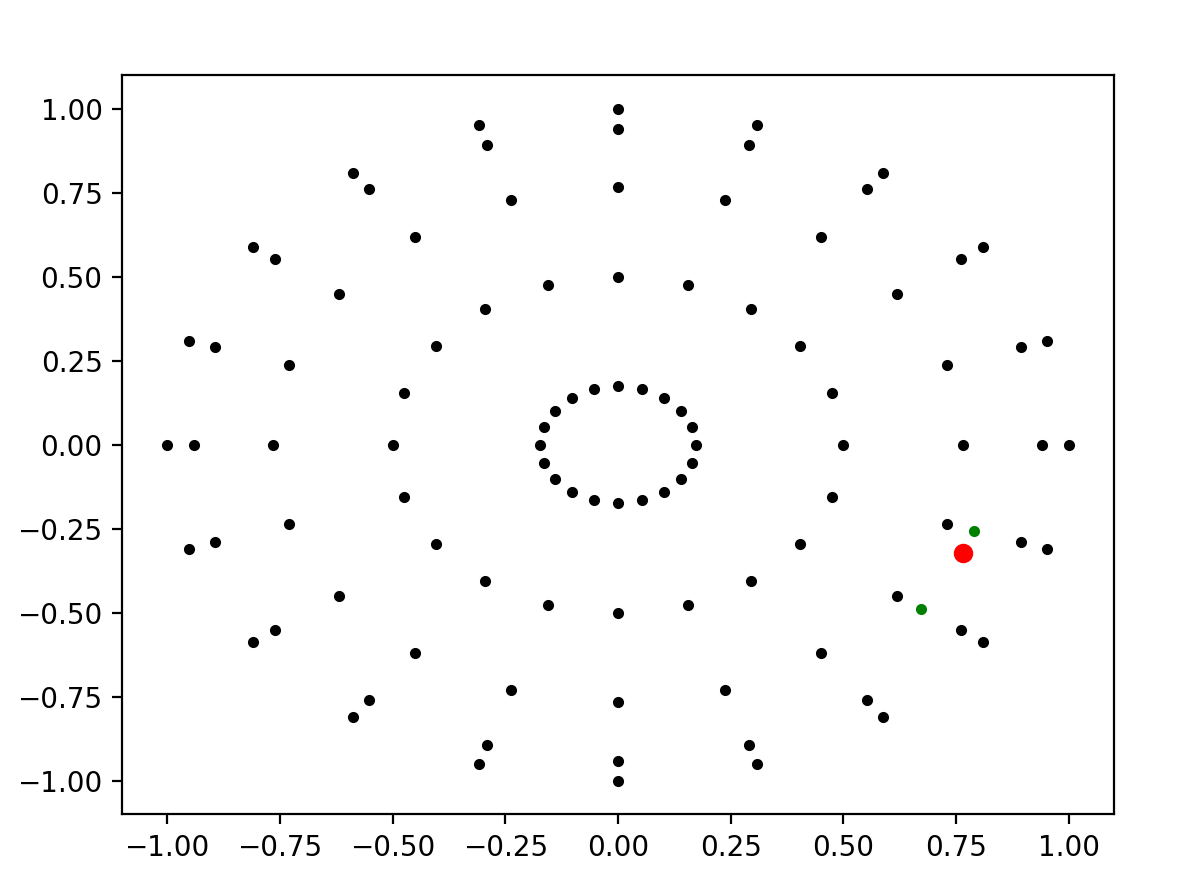
\includegraphics[width=0.8\textwidth]{StraddlePoints.jpg}
\caption{We want to find the red point. The green points are our straddle points. We need to find code to find the green points.}
\end{figure}

This should be a better method for accuracy since we are not looking for 4 points. \\

In order to code this, we need a 1-dimensional interpolation scheme. We want the interpolation scheme to be fast to evaluate and stable. 

\begin{align*}
P_n(x) = \frac{{\sum_{j = 0}^{n}}' \frac{(-1)^j f_j}{x-x_j}}{{\sum_{j = 0}^{n}}' \frac{(-1)^j}{x-x_j}} \\
{\sum _{j = 0}^{n}}' = \frac{1}{2}(j = 0) + (j = 1) + \dots + \frac{1}{2}(j = n)
\end{align*}

In the above equations, the x is equivalent to the s-value and the f is equivalent to the corresponding function value. A way to easier code the summation would be to rewrite it with normal summations.

\begin{align*}
P_n(x) = \frac{\sum_{j = 0}^{n} \alpha_j \frac{f_j}{x-x_j}}{\sum_{j = 0}^{n} \alpha_j\frac{1}{x-x_j}} \\
\alpha_0 = \frac{1}{2},\quad \alpha_{1:n-1} = (-1)^{1:n-1},\quad \alpha_n = \frac{1}{2} (-1)^n
\end{align*}